\documentclass[11pt,a4paper,fontset=none]{ctexart}
\usepackage{fontspec}
\usepackage{xeCJK}
\usepackage{amsmath,amssymb,mathtools}
\usepackage{geometry}
\usepackage[dvipsnames]{xcolor}
\usepackage{tikz}
\usetikzlibrary{
  arrows.meta,
  angles,
  backgrounds,
  calc,
  decorations.markings,
  decorations.pathmorphing,
  decorations.pathreplacing,
  fit,
  intersections,
  matrix,
  patterns,
  patterns.meta,
  positioning,
  quotes,
  shapes.geometric,
  shapes.misc,
  through,
  3d
}
\usepackage{pgfplots}
\pgfplotsset{compat=1.18}
\usepackage[most]{tcolorbox}
\usepackage{enumitem}
\usepackage{multicol}
\usepackage{tabularx,array,booktabs,multirow}
\usepackage{fancyhdr}
\usepackage{lastpage}
\usepackage{titlesec}
\usepackage{needspace}
\usepackage{eso-pic}
\usepackage{graphicx}
\usepackage{hyperref}
\usepackage{xparse}

\geometry{
  a4paper,
  left=18mm,
  right=18mm,
  top=22mm,
  bottom=20mm,
  headheight=22pt,
  headsep=8mm,
  footskip=11mm
}

\setmainfont{texgyrepagella-regular.otf}[
  BoldFont=texgyrepagella-bold.otf,
  ItalicFont=texgyrepagella-italic.otf,
  BoldItalicFont=texgyrepagella-bolditalic.otf
]
\setsansfont{texgyreheros-regular.otf}[
  BoldFont=texgyreheros-bold.otf,
  ItalicFont=texgyreheros-italic.otf,
  BoldItalicFont=texgyreheros-bolditalic.otf
]
\setmonofont{texgyrecursor-regular.otf}[
  BoldFont=texgyrecursor-bold.otf
]
\setCJKmainfont{Kaiti SC}[
  BoldFont=Kaiti SC
]
\setCJKsansfont{FandolHei-Regular.otf}[
  BoldFont=FandolHei-Bold.otf
]
\setCJKmonofont{FandolKai-Regular.otf}

\definecolor{Paper}{HTML}{FBFCFA}
\definecolor{Ink}{HTML}{17324D}
\definecolor{Muted}{HTML}{647784}
\definecolor{Teal}{HTML}{167D89}
\definecolor{TealDark}{HTML}{0F5F69}
\definecolor{Mint}{HTML}{E8F5F2}
\definecolor{Sky}{HTML}{EAF3F8}
\definecolor{Coral}{HTML}{E66A5A}
\definecolor{Gold}{HTML}{D7A94A}
\definecolor{Rule}{HTML}{C8D8DA}
\definecolor{SolutionBg}{HTML}{FFF9F1}

\pagecolor{Paper}
\color{Ink}
\linespread{1.14}
\setlength{\parindent}{2em}
\setlength{\parskip}{0.25em}
\setlength{\columnsep}{1.3cm}
\setlength{\abovedisplayskip}{0.7em}
\setlength{\belowdisplayskip}{0.7em}
\setlist{nosep}

\hypersetup{
  colorlinks=true,
  linkcolor=TealDark,
  urlcolor=TealDark,
  pdfborder={0 0 0}
}

\newcommand{\papertitle}{Mathstalents 小学版练习题}
\newcommand{\SetPaperTitle}[1]{\renewcommand{\papertitle}{#1}}

\pagestyle{fancy}
\fancyhf{}
\fancyhead[L]{\sffamily\small\color{TealDark}\papertitle}
\fancyhead[R]{}
\fancyfoot[C]{%
  {\sffamily\scriptsize\color{Muted}第~\arabic{page}~页~/~共~\pageref*{LastPage}~页}%
}
\renewcommand{\headrulewidth}{0.4pt}
\renewcommand{\footrulewidth}{0pt}
\renewcommand{\headrule}{\hbox to\headwidth{\color{Rule}\leaders\hrule height \headrulewidth\hfill}}

\AddToShipoutPictureBG{%
  \begin{tikzpicture}[remember picture,overlay]
    \draw[Rule,line width=0.35pt,rounded corners=2pt]
      ([xshift=6mm,yshift=-6mm]current page.north west)
      rectangle
      ([xshift=-6mm,yshift=6mm]current page.south east);
    \draw[Teal,line width=1.1pt]
      ([xshift=6mm,yshift=-14mm]current page.north west) --
      ([xshift=6mm,yshift=-6mm]current page.north west) --
      ([xshift=14mm,yshift=-6mm]current page.north west);
    \draw[Coral,line width=1.1pt]
      ([xshift=-6mm,yshift=14mm]current page.south east) --
      ([xshift=-6mm,yshift=6mm]current page.south east) --
      ([xshift=-14mm,yshift=6mm]current page.south east);
  \end{tikzpicture}%
}

\newcommand{\metachip}[2][Teal]{%
  \tikz[baseline=(chip.base)]\node[
    fill=#1!10,
    draw=#1!45,
    text=#1!80!black,
    rounded corners=2.5pt,
    inner xsep=6pt,
    inner ysep=2.4pt,
    font=\sffamily\scriptsize
  ] (chip) {\textbf{#2}};%
}

\NewDocumentCommand{\makecover}{m m m m m m}{%
  \thispagestyle{empty}
  \begin{tikzpicture}[remember picture,overlay]
    \draw[Teal!14,line width=0.8pt,step=10mm]
      ([xshift=8mm,yshift=8mm]current page.south west) grid
      ([xshift=-8mm,yshift=-8mm]current page.north east);
    \node[
      anchor=north west,
      text=Ink,
      align=left,
      text width=155mm
    ] at ([xshift=24mm,yshift=-35mm]current page.north west) {
      {\sffamily\bfseries\fontsize{14}{18}\selectfont
        MATHSTALENTS \(\cdot\) ELEMENTARY}\\[9mm]
      {\sffamily\bfseries\fontsize{34}{42}\selectfont
        小学版 \(\,\boldsymbol{\cdot}\,\) #1}\\[3mm]
      {\sffamily\fontsize{17}{23}\selectfont
        练习题与参考答案}\\[11mm]
      {\color{TealDark}\rule{112mm}{1.1pt}}\\[7mm]
      {\sffamily\fontsize{13}{20}\selectfont #2}
    };
    \node[
      anchor=north west,
      fill=white,
      draw=TealDark,
      line width=0.6pt,
      text opacity=1,
      rounded corners=5pt,
      inner sep=9mm,
      text width=137mm
    ] at ([xshift=24mm,yshift=-126mm]current page.north west) {
      \begin{minipage}{137mm}
        \sffamily
        \begin{tabularx}{\linewidth}{>{\centering\arraybackslash}X
          >{\centering\arraybackslash}X
          >{\centering\arraybackslash}X}
          {\color{TealDark}\bfseries\Large #3} &
          {\color{TealDark}\bfseries\Large #4} &
          {\color{TealDark}\bfseries\Large 精编}\\[-1mm]
          {\color{Muted}\small 总分} &
          {\color{Muted}\small 题目数} &
          {\color{Muted}\small 题解版本}
        \end{tabularx}
        \vspace{6mm}
        {\color{Rule}\hrule}
        \vspace{5mm}
        {\color{Ink}\bfseries 题型结构}\par
        \vspace{2mm}
        {\color{Muted}\small #5}
      \end{minipage}
    };
  \end{tikzpicture}
  \null
  \clearpage
}

\newcommand{\paperinfo}[3]{%
  \begin{tcolorbox}[
    enhanced,
    colback=Sky,
    colframe=Teal!40,
    boxrule=0.6pt,
    arc=3pt,
    left=5mm,right=5mm,top=4mm,bottom=4mm
  ]
    \sffamily
    \begin{tabularx}{\linewidth}{@{}X X X@{}}
      \textbf{姓名：}\rule{28mm}{0.4pt} &
      \textbf{用时：}\rule{22mm}{0.4pt} &
      \textbf{得分：}\rule{22mm}{0.4pt}\\[3mm]
      \multicolumn{3}{@{}l@{}}{\small\color{Muted}
        #1 \qquad #2 \qquad #3}
    \end{tabularx}
  \end{tcolorbox}
  \vspace{2mm}
}

\newcommand{\mtQuestionNeedspace}{8.2cm}
\newcommand{\mtBannerNeedspace}{6.8cm}
\newcommand{\mtQuestionBreakLines}{8}

\newcommand{\sectionbanner}[2]{%
  \Needspace{\mtBannerNeedspace}
  \begin{tcolorbox}[
    enhanced,
    colback=white,
    colframe=TealDark,
    boxrule=0.65pt,
    arc=2.5pt,
    left=4mm,right=4mm,top=2.6mm,bottom=2.6mm,
    before skip=3.2mm,
    after skip=2.2mm
  ]
    {\sffamily\bfseries\large\color{TealDark}#1\quad
     \sffamily\small #2}
  \end{tcolorbox}
}

\NewDocumentEnvironment{question}{m m}{%
  \Needspace{\mtQuestionNeedspace}
  \begin{tcolorbox}[
    enhanced,
    breakable,
    lines before break=\mtQuestionBreakLines,
    colback=white,
    colframe=Rule,
    boxrule=0.55pt,
    arc=3pt,
    left=5mm,right=5mm,top=5mm,bottom=4mm,
    before skip=4mm,
    after skip=4mm,
    title={\sffamily\bfseries 第 #1 题（ #2 分 ）},
    coltitle=TealDark,
    colbacktitle=white,
    fonttitle=\sffamily\bfseries,
    attach boxed title to top left={xshift=4mm,yshift=-2.8mm},
    boxed title style={
      colback=white,
      colframe=TealDark,
      arc=2.5pt,
      boxrule=0.65pt,
      left=3mm,right=3mm,top=1.5mm,bottom=1.5mm
    }
  ]
  \hypertarget{question:#1}{}%
  \vspace{1mm}
}{%
  \end{tcolorbox}
}

\ExplSyntaxOn
\seq_new:N \g_mt_choices_seq
\dim_new:N \l_mt_choice_max_dim
\dim_new:N \l_mt_choice_sum_dim
\dim_new:N \l_mt_choice_tmp_dim
\dim_new:N \l_mt_choice_label_dim
\box_new:N \l_mt_choice_box

\NewDocumentCommand{\choice}{m}
{
  \seq_gput_right:Nn \g_mt_choices_seq {#1}
}

\cs_new_protected:Npn \mt_set_choice_label_dim:
{
  \hbox_set:Nn \l_mt_choice_box
  {
    \textcolor{TealDark}{\bfseries E.}
    \hspace{0.45em}
  }
  \dim_set:Nn \l_mt_choice_label_dim { \box_wd:N \l_mt_choice_box }
}

\cs_new_protected:Npn \mt_choice_label:n #1
{
  \textcolor{TealDark}{\bfseries \int_to_Alph:n {#1}.}
}

\cs_new_protected:Npn \mt_typeset_choice:nn #1#2
{
  \mt_choice_label:n {#1}\hspace{0.45em}#2
}

\cs_new_protected:Npn \mt_typeset_choice_par:nn #1#2
{
  \par\noindent
  \hangindent = \l_mt_choice_label_dim
  \hangafter = 1
  \makebox[\l_mt_choice_label_dim][l]{ \mt_choice_label:n {#1} }
  #2
  \par
}

\cs_new_protected:Npn \mt_measure_choices:
{
  \dim_zero:N \l_mt_choice_max_dim
  \dim_zero:N \l_mt_choice_sum_dim
  \int_step_inline:nn { \seq_count:N \g_mt_choices_seq }
  {
    \hbox_set:Nn \l_mt_choice_box
    {
      \mt_typeset_choice:nn {##1} { \seq_item:Nn \g_mt_choices_seq {##1} }
    }
    \dim_set:Nn \l_mt_choice_tmp_dim { \box_wd:N \l_mt_choice_box }
    \dim_set:Nn \l_mt_choice_sum_dim { \l_mt_choice_sum_dim + \l_mt_choice_tmp_dim + 1.6em }
    \dim_set:Nn \l_mt_choice_max_dim
    {
      \dim_max:nn { \l_mt_choice_max_dim } { \l_mt_choice_tmp_dim }
    }
  }
}

\cs_new_protected:Npn \mt_print_choices:
{
  \mt_set_choice_label_dim:
  \mt_measure_choices:
  \par\nopagebreak\vspace{0.5em}
  \dim_compare:nNnTF { \l_mt_choice_sum_dim } < { \linewidth }
  {
    \noindent
    \int_step_inline:nn { \seq_count:N \g_mt_choices_seq }
    {
      \mbox
      {
        \mt_typeset_choice:nn {##1} { \seq_item:Nn \g_mt_choices_seq {##1} }
      }
      \hfill
    }
    \par
  }
  {
    \dim_compare:nNnTF { \l_mt_choice_max_dim + 0.6em } < { 0.5\linewidth }
    {
      \noindent
      \int_step_inline:nn { \seq_count:N \g_mt_choices_seq }
      {
        \begin{minipage}[t]{0.48\linewidth}
          \raggedright
          \mt_typeset_choice_par:nn {##1} { \seq_item:Nn \g_mt_choices_seq {##1} }
        \end{minipage}
        \int_if_odd:nTF {##1}
        { \hfill }
        { \par\vspace{0.38em} }
      }
      \int_if_odd:nT { \seq_count:N \g_mt_choices_seq } { \par }
    }
    {
      \int_step_inline:nn { \seq_count:N \g_mt_choices_seq }
      {
        \mt_typeset_choice_par:nn {##1} { \seq_item:Nn \g_mt_choices_seq {##1} }
        \vspace{0.28em}
      }
    }
  }
  \vspace{0.25em}
  \seq_gclear:N \g_mt_choices_seq
}

\NewDocumentEnvironment{choices}{}
{
  \seq_gclear:N \g_mt_choices_seq
}
{
  \mt_print_choices:
}

\NewDocumentEnvironment{multichoices}{}
{
  \seq_gclear:N \g_mt_choices_seq
}
{
  \mt_print_choices:
}
\ExplSyntaxOff

\NewDocumentCommand{\subquestion}{m m}{%
  \par\medskip
  \noindent
  \metachip[Coral]{#1 分}\hspace{0.7em}#2\par
}

\newcommand{\answerlineskip}{9mm}

\newcommand{\answerspace}{%
  \par\vspace{12mm}%
}

\newcommand{\answerline}{%
  \ifmmode
    \underline{\hspace{2.8cm}}%
  \else
    \ifvmode
      \par\vspace{\answerlineskip}%
      \noindent{\color{Ink}\rule{0.46\linewidth}{0.5pt}}%
      \par\vspace{2.5mm}%
    \else
      \underline{\hspace{2.8cm}}%
    \fi
  \fi
}

\NewDocumentCommand{\answerbox}{m}{%
  \par\vspace{3mm}
  \begin{tcolorbox}[
    enhanced,
    colback=white,
    colframe=Teal!38!Rule,
    boxrule=0.7pt,
    arc=2.5pt,
    left=3.5mm,
    right=3.5mm,
    top=3mm,
    bottom=3mm,
    height=#1,
    before skip=0pt,
    after skip=2mm
  ]
    \mbox{}
  \end{tcolorbox}
}

\NewDocumentEnvironment{solution}{m m m m}{%
  \Needspace{5.4cm}
  \begin{tcolorbox}[
    enhanced,
    breakable,
    lines before break=6,
    colback=white,
    colframe=Gold!65!Ink,
    boxrule=0.6pt,
    arc=3pt,
    left=5mm,right=5mm,top=5mm,bottom=4mm,
    before skip=4mm,
    after skip=4mm,
    title={\sffamily\bfseries 第 #1 题 \(\cdot\) 参考解答},
    coltitle=Ink,
    colbacktitle=white,
    fonttitle=\sffamily\bfseries,
    attach boxed title to top left={xshift=4mm,yshift=-2.8mm},
    boxed title style={
      colback=white,
      colframe=Gold!65!Ink,
      arc=2.5pt,
      boxrule=0.65pt,
      left=3mm,right=3mm,top=1.5mm,bottom=1.5mm
    }
  ]
  \hypertarget{solution:#1}{}%
  \vspace{1mm}
  \noindent
  \metachip[Coral]{答案：#2}\hspace{0.45em}
  \metachip[Gold]{难度：#3}\hspace{0.45em}
  \metachip[Teal]{#4}
  \par\medskip
}{%
  \end{tcolorbox}
}

\NewDocumentCommand{\analysis}{+m}{%
  \par\smallskip
  {\sffamily\bfseries\color{TealDark}思路分析}\par
  \vspace{1mm}
  #1
  \par\smallskip
}

\NewDocumentCommand{\methodsummary}{+m}{%
  \par\medskip
  \noindent
  {\sffamily\bfseries\color{TealDark}方法总结}\quad
  {\sffamily\color{Ink}#1}\par
}

\newcommand{\solutiondivider}{%
  \clearpage
}


\SetPaperTitle{第五套卷 · 第17题第（3）问}
\hypersetup{
  pdftitle={第五套卷第17题第（3）问：反弹路线与六边形展开},
  pdfauthor={第17题第（3）问详解}
}

\tikzset{
  route/.style={Coral,line width=1.05pt,line cap=round,line join=round},
  hexedge/.style={Ink,line width=0.75pt,line cap=round,line join=round},
  hit/.style={Teal,line width=1.35pt,line cap=round,line join=round},
  guide/.style={Muted,densely dashed,line width=0.6pt},
  dimline/.style={Muted,line width=0.55pt,{Bar[width=3.2pt]}-{Bar[width=3.2pt]}},
  vtx/.style={circle,fill=Coral,inner sep=0pt,minimum size=3.4pt},
  roomtag/.style={font=\scriptsize,text=Muted,inner sep=1pt}
}

\begin{document}

\section*{第五套卷\quad 第17题第（3）问}

正六边形 \(ABCDEF\) 的边长为 \(1\,\mathrm{cm}\)。点从顶点 \(A\) 出发，在内部沿直线走；碰到一条边时按入射角等于反射角反弹，碰到顶点就停止。已知第一次反弹发生在边 \(CD\) 上。

第（3）问：点先在 \(CD\) 上的点 \(Y\) 反弹，接着再连续反弹两次（一共三次），最后正好到达顶点 \(D\)。求 \(CY\) 的长度。

\begin{center}
\renewcommand{\arraystretch}{1.15}
\begin{tabular}{cccc}
A & B & C & D\\
\(\dfrac{3}{5}\,\mathrm{cm}\) &
\(\dfrac{4}{7}\,\mathrm{cm}\) &
\(\dfrac{5}{7}\,\mathrm{cm}\) &
\(\dfrac{5}{8}\,\mathrm{cm}\)
\end{tabular}
\end{center}

答案是 \(\dfrac{5}{7}\,\mathrm{cm}\)，选 C。下面先把六边形里的折线、以及它在密铺展开图里对应的直线画出来，再按这张图完成计算。

\section*{一、六边形里的三次反弹}

图1是题目原来的朝向：\(A\) 在最上，\(D\) 在最下，\(CD\) 是左下斜边。折线为
\[
  A \longrightarrow Y \longrightarrow M \longrightarrow Z \longrightarrow D.
\]
\(Y\) 在 \(CD\) 上，\(M\) 是右边竖直边 \(EF\) 的中点，\(Z\) 在左上边 \(AB\) 上，并且 \(AZ=\dfrac{2}{7}\,\mathrm{cm}\)。走到 \(D\) 时碰到顶点，运动停止。这四个落点为什么必须是它们，要等展开图里的直线确定之后才能读出来；长度 \(CY=\dfrac{5}{7}\) 也在那里算。

\begin{center}
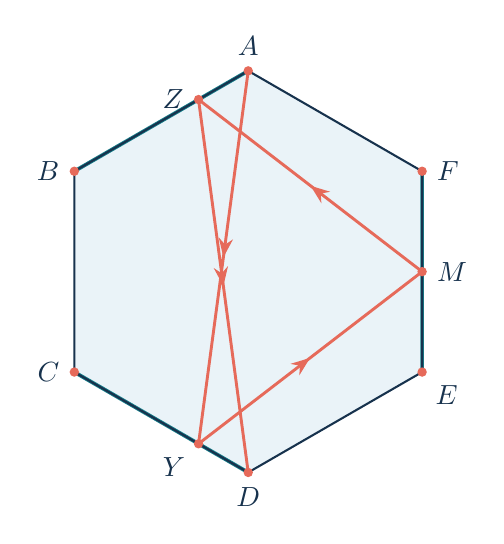
\begin{tikzpicture}[scale=2.55,>=Stealth]
  \coordinate (A) at (0,1);
  \coordinate (B) at ({-sqrt(3)/2},1/2);
  \coordinate (C) at ({-sqrt(3)/2},{-1/2});
  \coordinate (D) at (0,-1);
  \coordinate (E) at ({sqrt(3)/2},{-1/2});
  \coordinate (F) at ({sqrt(3)/2},1/2);
  \coordinate (Y) at ({-sqrt(3)/7},{-6/7});
  \coordinate (M) at ({sqrt(3)/2},0);
  \coordinate (Z) at ({-sqrt(3)/7},{6/7});

  \fill[Sky] (A)--(B)--(C)--(D)--(E)--(F)--cycle;
  \draw[hit] (C)--(D) (E)--(F) (A)--(B);
  \draw[hexedge] (A)--(B)--(C)--(D)--(E)--(F)--cycle;

  \draw[route,postaction={decorate},decoration={markings,
    mark=at position 0.143 with {\arrow{Stealth[length=2.4mm,width=1.8mm]}},
    mark=at position 0.393 with {\arrow{Stealth[length=2.4mm,width=1.8mm]}},
    mark=at position 0.607 with {\arrow{Stealth[length=2.4mm,width=1.8mm]}},
    mark=at position 0.857 with {\arrow{Stealth[length=2.4mm,width=1.8mm]}}
  }] (A)--(Y)--(M)--(Z)--(D);

  \node[vtx,label={[Ink]above:{\(A\)}}] at (A) {};
  \node[vtx,label={[Ink]left:{\(B\)}}] at (B) {};
  \node[vtx,label={[Ink]left:{\(C\)}}] at (C) {};
  \node[vtx,label={[Ink]below:{\(D\)}}] at (D) {};
  \node[vtx,label={[Ink]below right:{\(E\)}}] at (E) {};
  \node[vtx,label={[Ink]right:{\(F\)}}] at (F) {};
  \node[vtx,label={[Ink]below left:{\(Y\)}}] at (Y) {};
  \node[vtx,label={[Ink]right:{\(M\)}}] at (M) {};
  \node[vtx,label={[Ink]left:{\(Z\)}}] at (Z) {};
\end{tikzpicture}

\vspace{0.35em}
{\small\color{Ink}图1\quad 原六边形中的反弹路线。青色边是三次碰到的边 \(CD\)、\(EF\)、\(AB\)。}
\end{center}

\section*{二、密铺展开后的直线}

正六边形能铺满平面。把六边形沿一条边翻到旁边那一块，反弹就变成穿墙而过：入射角等于反射角，正好相当于镜子两边的路径连成一条直线。

三次反弹之后停在 \(D\)，对应直线穿过三面墙，终点是 \(D\) 的镜像 \(D_3\)。图2保持图1的朝向，四块六边形按反弹的顺序贴在一起：

\begin{enumerate}[leftmargin=1.7em,itemsep=0.28em]
  \item 沿 \(CD\) 翻出第 1 块，对应第一次反弹。
  \item 第 1 块朝原六边形 \(EF\) 的那条边再翻出第 2 块，对应第二次反弹。
  \item 第 2 块再沿对应 \(AB\) 的那条边翻出第 3 块。\(D_3\) 是这一块上 \(D\) 的像，直线走进这个顶点，对应第三次反弹之后到达 \(D\)。
\end{enumerate}

直线 \(AD_3\) 第一次穿墙的位置就是 \(Y\)。它后面两个穿墙点折回图1，分别是 \(M\) 和 \(Z\)。

\begin{center}
\begin{tikzpicture}[scale=1.28,>=Stealth]
  % room 0
  \coordinate (A) at (0,1);
  \coordinate (B) at ({-sqrt(3)/2},1/2);
  \coordinate (C) at ({-sqrt(3)/2},{-1/2});
  \coordinate (D) at (0,-1);
  \coordinate (E) at ({sqrt(3)/2},{-1/2});
  \coordinate (F) at ({sqrt(3)/2},1/2);
  % room 1
  \coordinate (A1) at ({-sqrt(3)},-2);
  \coordinate (B1) at ({-sqrt(3)},-1);
  \coordinate (E1) at (0,-2);
  \coordinate (F1) at ({-sqrt(3)/2},{-5/2});
  % room 2
  \coordinate (A2) at ({-sqrt(3)/2},{-7/2});
  \coordinate (B2) at (0,-4);
  \coordinate (C2) at ({sqrt(3)/2},{-7/2});
  \coordinate (D2) at ({sqrt(3)/2},{-5/2});
  % room 3
  \coordinate (C3) at (0,-5);
  \coordinate (D3) at ({-sqrt(3)/2},{-11/2});
  \coordinate (E3) at ({-sqrt(3)},-5);
  \coordinate (F3) at ({-sqrt(3)},-4);

  \coordinate (Y) at ({-sqrt(3)/7},{-6/7});
  \coordinate (Mp) at ({-sqrt(3)/4},{-9/4});
  \coordinate (Zp) at ({-5*sqrt(3)/14},{-51/14});

  \fill[Sky] (A)--(B)--(C)--(D)--(E)--(F)--cycle;
  \fill[Teal!12] (A1)--(B1)--(C)--(D)--(E1)--(F1)--cycle;
  \fill[Mint] (A2)--(B2)--(C2)--(D2)--(E1)--(F1)--cycle;
  \fill[Coral!12] (A2)--(B2)--(C3)--(D3)--(E3)--(F3)--cycle;

  \draw[hexedge] (A)--(B)--(C)--(D)--(E)--(F)--cycle;
  \draw[hexedge] (A1)--(B1)--(C)--(D)--(E1)--(F1)--cycle;
  \draw[hexedge] (A2)--(B2)--(C2)--(D2)--(E1)--(F1)--cycle;
  \draw[hexedge] (A2)--(B2)--(C3)--(D3)--(E3)--(F3)--cycle;

  \draw[route,postaction={decorate},decoration={markings,
    mark=at position 0.55 with {\arrow{Stealth[length=2.6mm]}}
  }] (A)--(D3);

  \node[roomtag] at (0.28,0.22) {原六边形};
  \node[roomtag] at (-1.05,-1.55) {第1块};
  \node[roomtag] at (0.38,-3.05) {第2块};
  \node[roomtag] at (-0.22,-4.55) {第3块};

  \node[font=\scriptsize,text=Ink,above] at (A) {\(A\)};
  \node[font=\scriptsize,text=Ink,left] at (B) {\(B\)};
  \node[font=\scriptsize,text=Ink,left] at (C) {\(C\)};
  \node[font=\scriptsize,text=Ink,below right] at (D) {\(D\)};
  \node[font=\scriptsize,text=Ink,right] at (E) {\(E\)};
  \node[font=\scriptsize,text=Ink,right] at (F) {\(F\)};
  \node[vtx,label={[font=\scriptsize,Ink]left:{\(Y\)}}] at (Y) {};
  \node[vtx,label={[font=\scriptsize,Ink]left:{\(M'\)}}] at (Mp) {};
  \node[vtx,label={[font=\scriptsize,Ink]below right:{\(Z'\)}}] at (Zp) {};
  \node[vtx,label={[font=\scriptsize,Ink]below:{\(D_3\)}}] at (D3) {};
  % images of the original vertices; a vertex on the mirror stays put
  \node[font=\scriptsize,text=TealDark,above left] at (B1) {\(B\)};
  \node[font=\scriptsize,text=TealDark,left] at (A1) {\(A\)};
  \node[font=\scriptsize,text=TealDark,below left] at (F1) {\(F\)};
  \node[font=\scriptsize,text=TealDark,right=2pt] at (E1) {\(E\)};
  \node[font=\scriptsize,text=TealDark,right] at (D2) {\(D\)};
  \node[font=\scriptsize,text=TealDark,right] at (C2) {\(C\)};
  \node[font=\scriptsize,text=TealDark,above left] at (A2) {\(A\)};
  \node[font=\scriptsize,text=TealDark,right=2pt] at (B2) {\(B\)};
  \node[font=\scriptsize,text=TealDark,left] at (F3) {\(F\)};
  \node[font=\scriptsize,text=TealDark,left] at (E3) {\(E\)};
  \node[font=\scriptsize,text=TealDark,right] at (C3) {\(C\)};
\end{tikzpicture}

\vspace{0.4em}
{\small\color{Ink}图2\quad 与图1同一朝向的展开。折线 \(AYMZD\) 变成直线 \(AD_3\)。青色字母是翻折后对应的原顶点：公共边上的字母不动，其余字母翻到对面。第 3 块最下方的 \(D_3\) 是 \(D\) 的像。\(M'\)、\(Z'\) 折回原六边形就是 \(M\)、\(Z\)。}
\end{center}

第二次若落在 \(AF\) 上，展开时直线会穿过第 1 块的底边，接着就走进 \(D\) 的另一个镜像。那条路线一共只反弹两次，是第（2）问，得到 \(CX=\dfrac{1}{3}\,\mathrm{cm}\)。第（3）问在到达 \(D\) 之前还要再反弹一次，所以第二次落在 \(EF\) 上，展开图进入右下方的第 2 块，再向下翻出第 3 块。

\section*{三、把 \(CD\) 放平后量 \(D_3\)}

图1里对角线 \(AC\) 垂直于 \(CD\)。把 \(CD\) 转成水平以后，\(A\) 就在 \(C\) 的正上方。两条平行边之间的距离记作 \(1\) 层；\(A\) 到 \(CD\) 正好是 \(1\) 层。横轴仍用厘米。图3是图2转过之后的同一条直线，尺寸都标在这张图上。

四块的中心可以顺着蜂巢数出来。以 \(C\) 为横轴原点，\(CD\) 的高度为 \(0\)，向上为正：

\begin{enumerate}[leftmargin=1.7em,itemsep=0.32em]
  \item 原六边形的中心在 \(CD\) 中点的正上方，所以它的横坐标是 \(0.5\)，高度是 \(+0.5\) 层。
  \item 第 1 块在 \(CD\) 正下方。中心横坐标仍是 \(0.5\)，高度是 \(-0.5\) 层。
  \item 第 2 块是第 1 块的右下邻居。斜向相邻两块的中心，横坐标相差 \(1.5\,\mathrm{cm}\)，高度再低 \(0.5\) 层。中心到了横坐标 \(2\)，高度 \(-1\) 层。
  \item 第 3 块在第 2 块正下方，横坐标仍是 \(2\)，高度再低 \(1\) 层，中心在 \(-2\) 层。
  \item \(D_3\) 是第 3 块的右下角，比该块中心再向右 \(0.5\,\mathrm{cm}\)、再向下 \(0.5\) 层。
\end{enumerate}

因此 \(D_3\) 在 \(C\) 的右方 \(2.5\,\mathrm{cm}\)，并且在 \(CD\) 下方 \(2.5\) 层。\(A\) 在 \(CD\) 上方 \(1\) 层，横坐标与 \(C\) 相同。

\begin{center}
\begin{tikzpicture}[scale=1.38,>=Stealth]
  \coordinate (A) at (-1/2,{sqrt(3)/2});
  \coordinate (B) at (-1,0);
  \coordinate (C) at (-1/2,{-sqrt(3)/2});
  \coordinate (D) at (1/2,{-sqrt(3)/2});
  \coordinate (E) at (1,0);
  \coordinate (F) at (1/2,{sqrt(3)/2});
  \coordinate (A1) at (-1/2,{-3*sqrt(3)/2});
  \coordinate (B1) at (-1,{-sqrt(3)});
  \coordinate (E1) at (1,{-sqrt(3)});
  \coordinate (F1) at (1/2,{-3*sqrt(3)/2});
  \coordinate (A2) at (1,{-2*sqrt(3)});
  \coordinate (B2) at (2,{-2*sqrt(3)});
  \coordinate (C2) at (5/2,{-3*sqrt(3)/2});
  \coordinate (D2) at (2,{-sqrt(3)});
  \coordinate (C3) at (5/2,{-5*sqrt(3)/2});
  \coordinate (D3) at (2,{-3*sqrt(3)});
  \coordinate (E3) at (1,{-3*sqrt(3)});
  \coordinate (F3) at (1/2,{-5*sqrt(3)/2});
  \coordinate (Y) at (3/14,{-sqrt(3)/2});
  \coordinate (H) at (-1/2,{-3*sqrt(3)});
  \coordinate (P2) at (3/4,{-5*sqrt(3)/4});
  \coordinate (P3) at (9/7,{-2*sqrt(3)});

  \fill[Sky] (A)--(B)--(C)--(D)--(E)--(F)--cycle;
  \fill[Teal!12] (A1)--(B1)--(C)--(D)--(E1)--(F1)--cycle;
  \fill[Mint] (A2)--(B2)--(C2)--(D2)--(E1)--(F1)--cycle;
  \fill[Coral!12] (A2)--(B2)--(C3)--(D3)--(E3)--(F3)--cycle;

  \draw[hexedge] (A)--(B)--(C)--(D)--(E)--(F)--cycle;
  \draw[hexedge] (A1)--(B1)--(C)--(D)--(E1)--(F1)--cycle;
  \draw[hexedge] (A2)--(B2)--(C2)--(D2)--(E1)--(F1)--cycle;
  \draw[hexedge] (A2)--(B2)--(C3)--(D3)--(E3)--(F3)--cycle;

  \draw[guide] (A)--(H);
  \draw[guide] (H)--(D3);
  \draw[route] (A)--(D3);

  % right angle at C: AC vertical, CD horizontal
  \draw[TealDark,line width=0.65pt]
    ($(C)+(0,0.20)$) -- ($(C)+(0.20,0.20)$) -- ($(C)+(0.20,0)$);

  \node[roomtag] at (0.05,0.08) {原六边形};
  \node[roomtag] at (-0.15,-1.62) {第1块};
  \node[roomtag] at (1.85,-2.35) {第2块};
  \node[roomtag] at (0.92,-4.55) {第3块};

  \node[font=\scriptsize,text=Ink,above] at (A) {\(A\)};
  \node[font=\scriptsize,text=Ink,left] at (B) {\(B\)};
  \node[font=\scriptsize,text=Ink,below left] at (C) {\(C\)};
  \node[font=\scriptsize,text=Ink,below] at (D) {\(D\)};
  \node[font=\scriptsize,text=Ink,right] at (E) {\(E\)};
  \node[font=\scriptsize,text=Ink,above] at (F) {\(F\)};
  \node[vtx,label={[font=\scriptsize,Ink]above right:{\(Y\)}}] at (Y) {};
  \node[vtx,label={[font=\scriptsize,Ink]above right:{\(M'\)}}] at (P2) {};
  \node[vtx,label={[font=\scriptsize,Ink]above:{\(Z'\)}}] at (P3) {};
  \node[vtx,label={[font=\scriptsize,Ink]right:{\(D_3\)}}] at (D3) {};
  \node[font=\scriptsize,text=Ink,below left] at (H) {\(H\)};

  \draw[dimline] (-1.55,{sqrt(3)/2}) -- (-1.55,{-sqrt(3)/2})
    node[midway,left,font=\scriptsize,text=Ink] {\(1\) 层};
  \draw[dimline] (-1.55,{-sqrt(3)/2}) -- (-1.55,{-3*sqrt(3)})
    node[midway,left,font=\scriptsize,text=Ink] {\(2.5\) 层};
  \draw[guide] (A) -- (-1.55,{sqrt(3)/2});
  \draw[guide] (C) -- (-1.55,{-sqrt(3)/2});
  \draw[guide] (H) -- (-1.55,{-3*sqrt(3)});

  \draw[dimline] (-1/2,{-3*sqrt(3)-0.42}) -- (2,{-3*sqrt(3)-0.42})
    node[midway,below,font=\scriptsize,text=Ink] {\(2.5\,\mathrm{cm}\)};
  \draw[guide] (H) -- (-1/2,{-3*sqrt(3)-0.42});
  \draw[guide] (D3) -- (2,{-3*sqrt(3)-0.42});
\end{tikzpicture}

\vspace{0.45em}
{\small\color{Ink}图3\quad 将 \(CD\) 置于水平后的同一条直线。\(A\) 在 \(C\) 正上方，直角标在 \(C\)。虚线 \(AH\)、\(HD_3\) 是用来做比例的直角三角形。}
\end{center}

\section*{四、用高度比求 \(CY\)}

把图3的坐标写成：横轴以 \(C\) 为 \(0\)，单位厘米；纵轴以 \(CD\) 为 \(0\)，向上为正，单位是层。于是
\[
  A=(0,\,1),\qquad D_3=(2.5,\,-2.5).
\]
连接它们的直线可以写成
\[
  x=2.5\,s,\qquad y=1-3.5\,s,\qquad 0\le s\le 1.
\]
参数 \(s=0\) 在 \(A\)，\(s=1\) 在 \(D_3\)。直线落到 \(CD\)（也就是 \(y=0\)）时，
\[
  1-3.5\,s=0,\qquad s=\frac{1}{3.5}=\frac{2}{7}.
\]
这一点的横坐标就是 \(CY\)，因为直线从 \(C\) 的正上方出发：
\[
  CY=2.5\times\frac{2}{7}=\frac{5}{2}\times\frac{2}{7}=\frac{5}{7}\,\mathrm{cm}.
\]

同一个比例可以看成直角三角形 \(AHD_3\) 和它被 \(CD\) 截出的小直角三角形。大三角形竖直 \(3.5\) 层、水平 \(2.5\,\mathrm{cm}\)；截到 \(CD\) 时竖直只走了 \(1\) 层，所以水平也只走了全程的 \(\dfrac{2}{7}\)。

把 \(s=\dfrac{2}{7}\) 代回直线，还可以读出另外两次穿墙的位置，折回图1就是：
\[
  M\text{ 为 }EF\text{ 的中点},\qquad AZ=\frac{2}{7}\,\mathrm{cm}.
\]
此后直线进入 \(D_3\)，对应点在原六边形里进入顶点 \(D\) 并停止。

\begin{tcolorbox}[
  colback=Mint,
  colframe=TealDark,
  boxrule=0.6pt,
  arc=2pt,
  left=8pt,right=8pt,top=6pt,bottom=6pt
]
\textbf{答案.}\quad \(CY=\dfrac{5}{7}\,\mathrm{cm}\)，选 C。
\end{tcolorbox}

\end{document}
